\section{Project methodology}
As mentioned earlier, the team chose Scrum as its project management framework. This section aims to explain how and why Scrum was used, and what issues that were encountered during the project. Even though Scrum is well known, many team members had different expectations to how the framework would be implemented in the project. It also describes how XP was adapted by the team members.

\subsection{Our adaptation of Scrum}



\subsection{Our adaptation of Extreme Programming}
Several modifications and adaptations were made to the Extreme Programming method in order to optimize it to fit the team's needs.

\paragraph{Pair programming}
The team has practised this principle by dividing the team into small groups or pairs when designing prototypes, deciding on architecture and in a few cases, collaborated on code sections.

\paragraph{Planning game}
The team interpreted the planning game in XP to be a more generic description of planning methods. We therefore argue that planning poker, which the team used for estimating the tasks, is a more specific implementation of the planning game in XP. Amongst other, one of the most important aspects of planning poker is that no team member should not know what the rest of the team choose to estimate in order to avoid the influence of the other participants. This aspect is not mentioned in the planning game specification in XP.

\paragraph{Continuous integration and collective ownership}
The team has practised this principle by working on code on separate branches in Git and merged these branches in a master-branch when a task was considered to be completed.

The team has also practised the collective ownership principle by sharing and collaborating on the project's code on GitHub. In addition, we agreed with the customer on following the Java code convention and Android code convention in the development.

\paragraph{Design improvement and optimization}
The team has continuously followed this practice and also practised it during design improvements in the development of prototypes.
 
\paragraph{Small releases}
The team has followed this practice by having sprints with a duration of two weeks, with a release for each sprint.


\paragraph{Simple design}
Although the team worked iteratively and in close collaboration with the customer, it has not always been easy to \emph{only} implement the basic functionality the customer requested. The initial assignment was very open for interpretation, and because it was the team's task to define the requirements specification, it was hard not to try to add functionality that we sincerely thought would improve the application, \todo{even though that functionality might not had been marked as a high priority assignment.problem: vi har ikke satt prioritet på alle oppgavene..}

\paragraph{Sustainable pace}
The team has practised this by having an estimation process where the amount of work hours were set to twenty hours a week.

\paragraph{On-site customer}
This principle does not apply to the team's project, as our customer comes from an external organization. However, we were co-located with our customer at a regular basis, usually once a week and hence got continuous feedback and acceptance testing.\todo{henvise til iterativ testing i testing-kapittelet}

\paragraph{Test-first development}
The team has not followed this practice. Although we initially thought it would be a good idea to have a test-driven development approach towards the testing process, the team quickly realized that we both lacked the experience and the time to follow this practice and therefore chose to drop it.




\subsection{Improper use of Yodiz}
\label{sec:improperScrum}
As mentioned in section~\ref{sec:scrumtool}, the team used a lot of time on
deciding on which Scrum tool to use for the project management. Although our
choice fell on Yodiz, the team was in lack of any previous experience with the
tool, and despite the team's efforts to get acquainted with the tool, a
misunderstanding arose and was not discovered until the end of the second
sprint.

The misunderstanding, displayed in figure~\ref{fig:wrongUse}, was that the team
assumed one could add multiple individuals as responsible on a particular task,
while Yodiz' functionality only assigned the time spent to the individual that
either created the task or was assigned as owner of the task.

As a result, it appeared as if only singular individuals performed the tasks,
even though the entire team in reality was participating, which was also
reflected in the burndown charts and the generated gantt diagram. 

To sort out this issue, the team went through old meeting reports and time sheets
to figure out which members of the team that had actually participated on the
particular task, and added new tasks and the time spent to the members that at
the time had not recorded this information, as shown in
figure~\ref{fig:addsTasks}.

This issue was unfortunate, but not insurmountable, and also not a critical
issue for the overall progress of the project.

\begin{figure}[H]
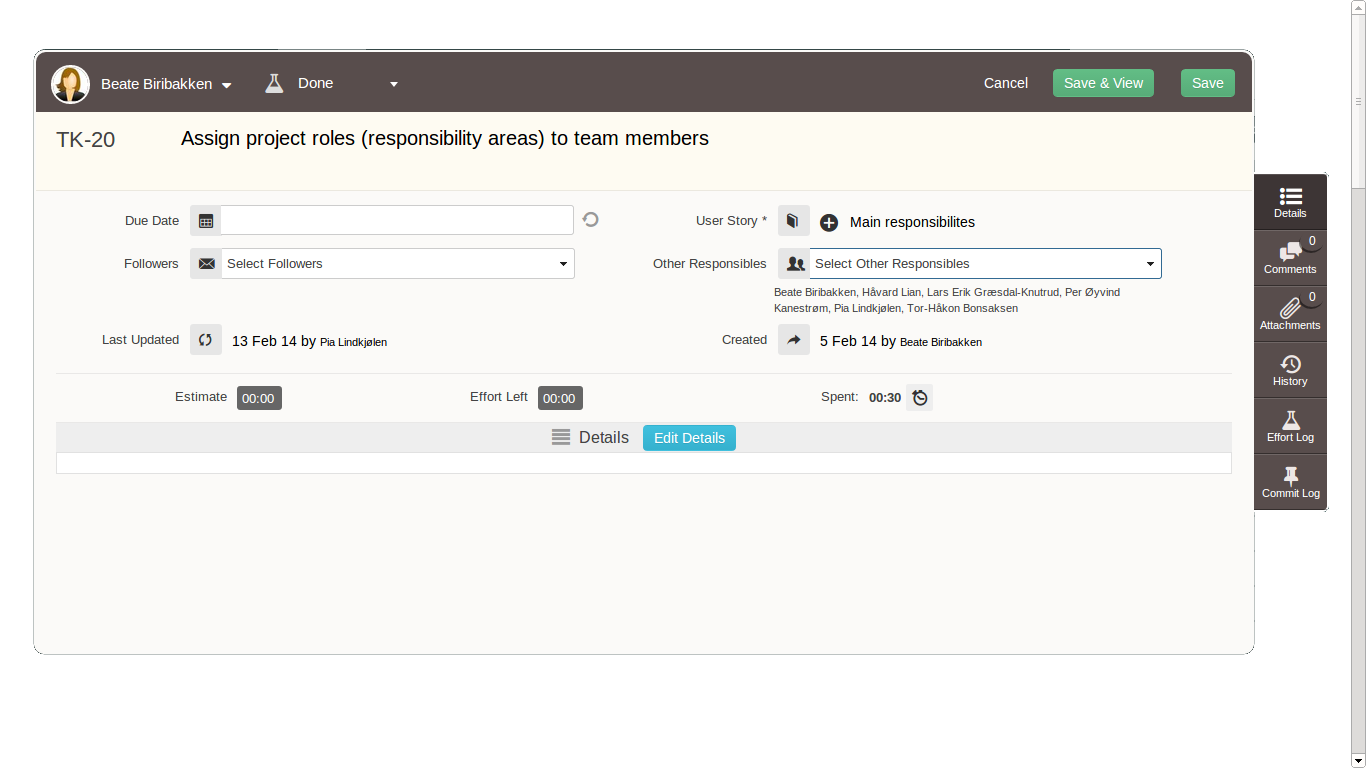
\includegraphics[width=\textwidth]{ch/devProcess/fig/wrongUse.png}
\caption{Example screenshot to illustrate improper use of Yodiz}
\label{fig:wrongUse}
\end{figure}

\begin{figure}[H]
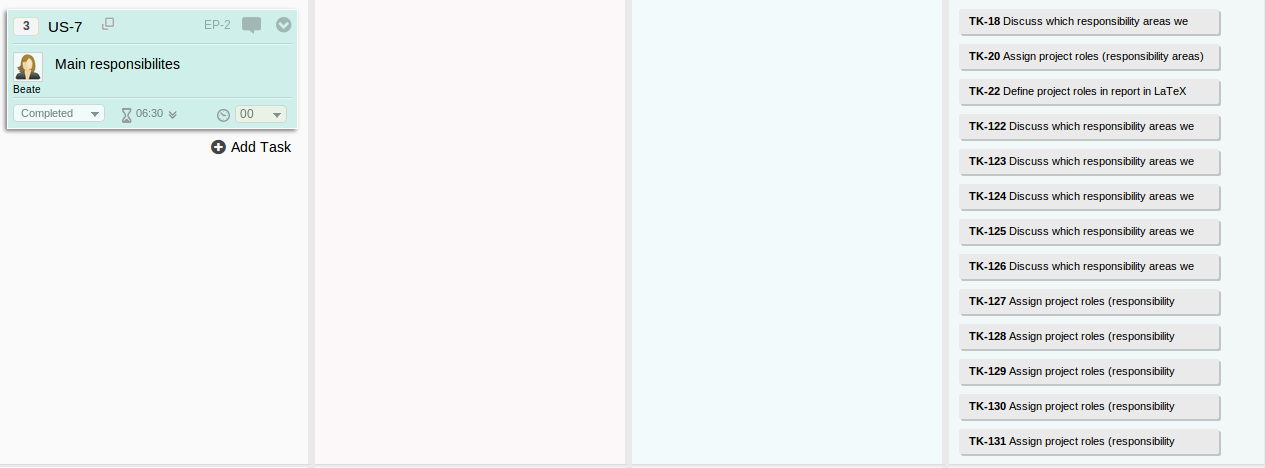
\includegraphics[width=\textwidth]{ch/devProcess/fig/addsTasks.png}
\caption{Example screenshot to illustrate how the team resolved the issue.}
\label{fig:addsTasks}
\end{figure}